\section{Description and Methodology}

This report describes three distinct systems; Each one more more power efficient than the last.

The first implementation is a simple polling-based approach. The second one uses interrupts, removing time needlessly used for idling. The final system goes into a deep sleep mode, waking only when coerced to do so by an interrupt from the GPIO controller.

Energy consumption was noted for each improvement to the system, and one can clearly see how power consumption is reduced by multiple orders of magnitude in the final system.

\subsection{A program without interrupts}

The first system implements a simple polling-based mechanism for updating the LEDs on the game pad. The main loop simply loads whatever values are found on the game pad (GPIO port C, pins 0-7), shifts them to the appropriate position required by the output port (GPIO port A, pins 8 - 15), and sets the corresponding pins to logical low.

\subsection{A program with interrupts}

The second system contains a simple, yet important architectural change. The system no longer blindly loads register values each tick, instead updating only when receiving interrupts from GPIO port C.

A number of flags are set to allow for interrupt-driven event handling, which are described in the following code segment \ref{lstinputlisting:interrupt-flags}.

Highlights include allowing for interrupt generation and -acceptance on GPIO port C, edge-driven interrupts on both hi-lo and lo-hi transitions from the gamepad, as well as enabling both odd and even interrupts.

\lstinputlisting[linerange={113-125}]{../code/ex1.s}
\label{lstinputlisting:interrupt-flags}

Callback handlers are registered for both odd and even pins. These allow us to handle the interrupts generated by the gamepad buttons.

\lstinputlisting[linerange={33-33, 43-43}]{../code/ex1.s}
\label{lstinputlisting:interrupt-handlers}

The interrupt handler is defined as folows \ref{lstinputlisting:interrupt-handler}.

First order of the day is clearing any potential lingering interrupts. This to avoid the interrupt handler being interrupted by another interrupt, hindering anything productive from being done.
Gamepad output is then loaded from GPIO port C, stored, bitshifted to match the output pins on port A, and written to the registry.

We use the fact that we have interrupts for both edge transitions on the gamepad available to set and clear the LEDs. This ensures that the LEDs are updated on both button presses- and releases. This contrasts with the earlier polling approach, where the values were blindly copied each tick.


\lstinputlisting[linerange={151-156, 162-170}]{../code/ex1.s}
\label{lstinputlisting:interrupt-handler}

\subsection{A program using low energy modes}
To save energy while running the program, it can use a low energy mode.
There are five different energy modes that can be used, with different peripherals available, as can be seen in figure \ref{fig:energy_modes}.\cite{referencemanual}

\begin{figure}[H]
\centering
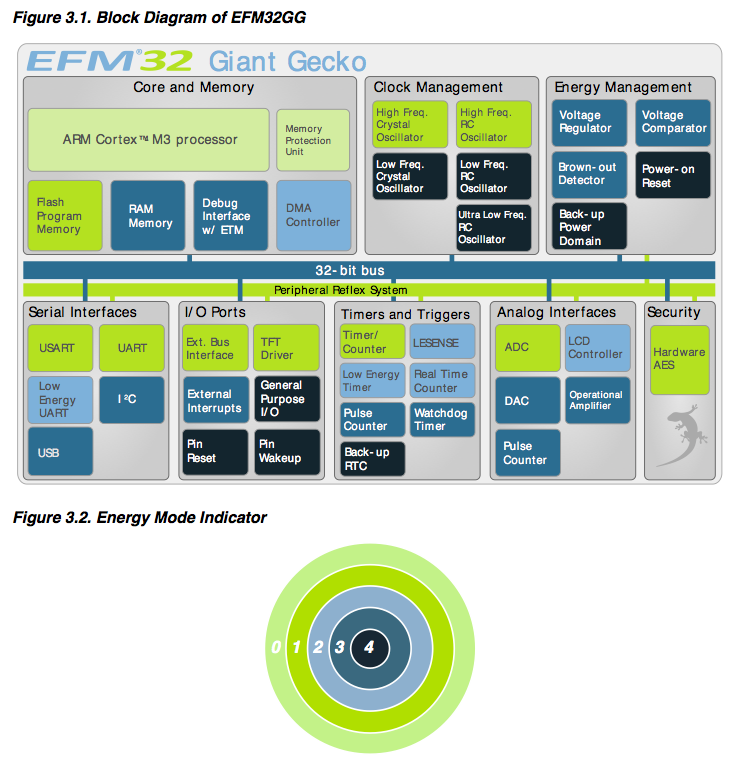
\includegraphics[scale=0.3]{figures/energymodes.png}
\caption{The different energy modes and available peripherals}
\label{fig:energy_modes}
\end{figure}

The trade off to use a low energy mode is that it uses some time to wake up (that is go from current energy mode to EM0)
From EM2 and EM3  the wake up time is about 2 $\mu$s, while in EM4 it is 160 $\mu$s.
EM1 has none latency.
For the user, a 0.1 s latency would feel instantaneous.\cite{response}
This means that even EM4 is satisfactory for the application, as after waking up from this mode will feel fast.

The only thing that needs to be done while the application is sleeping, is to wait for interrupts on the GPIO ports.
This excludes EM4, as to wake up from this mode with interrupts is only supported on a small number of GPIO ports.

Thus the deepest sleep the application can use is EM3.

\lstinputlisting[caption={Sleep mode enabling},label={lst:sleep},linerange={127-130}]{../code/ex1.s}

In listing \ref{lst:sleep}, energy mode 3 is enabled when the wait for instruction (wfi) instruction is called, or the code returns from an interrupt.
The wfi instruction is called in listing \ref{lst:loop}, the main loop of the program. 
This means that each time the program returns from an interrupt, wfi is 

\lstinputlisting[caption={Main loop}, label={lst:loop}, linerange={133-142}]{../code/ex1.s}
\subsubsection{Further improvements}

With these limitations, it is clear that the deep sleep mode will not be usable within the requirements and with the provided hardware.
A small change to the hardware would let the program work as intended, and sleep deeper.
With a multiplexer of all the signals from the buttons, and output to one of the supported GPIO ports, it would be easy to support EM4.
